%%+++++++++++++++++++++++++++++++++++++%%
%%         Final Version  6/14/95      %%
%%+++++++++++++++++++++++++++++++++++++%%
\documentclass[12pt]{article}
\textheight = 8.6in
\textwidth = 6.2in
\topmargin = -.5in
\oddsidemargin = 0.08in
\evensidemargin = 0.08in
%\usepackage{fancyhdr}
%\pagestyle{fancy}
%\rfoot{\thepage}
\setlength{\jot}{10.0 pt}
\setlength{\parskip}{2.5ex}
\setlength{\footskip}{65pt}

\usepackage{graphicx}
\usepackage{subfigure}
\usepackage{placeins}
\usepackage{afterpage}
\usepackage{amsmath}
\usepackage{empheq}
\usepackage[most]{tcolorbox}
\newtcbox{\mymath}[1][]{%
    nobeforeafter, math upper, tcbox raise base,
    enhanced, colframe=white!20!black ,
    colback=blue!30!red!30!white, boxrule=1pt,
    #1}
\usepackage{xcolor}
\definecolor{myblue}{RGB}{0, 0, 180}   %Numbers are integers from 0 to 255, smaller is closer to black
\definecolor{grey}{RGB}{200, 200, 200}   %Numbers are integers from 0 to 255, smaller is closer to black
\definecolor{mygreen}{RGB}{0, 80, 0}   %Numbers are integers from 0 to 255, smaller is closer to black
\definecolor{myred}{RGB}{120, 0, 0}   %Numbers are integers from 0 to 255, smaller is closer to black

\begin{document}

\begin{flushright} {\color{blue} Fourier Transforms} \end{flushright}
\begin{flushleft}

\subsubsection*{\color{myblue} {Complex Fourier Series} }

We are going to go through the following progression:
\[
\text{Fourier series} \hspace{.2in} \longrightarrow \hspace{.2in} \text{Complex Fourier Series} \hspace{.2in} \longrightarrow \hspace{.2in} \text{Fourier Transform}
\]

Last semester, our studies of expansions with orthogonal functions included the Fourier series expansion for a repeat interval $L$, 

\begin{equation}
f(x) = \frac{a_{0}}{2} + \sum_{n=1}^{\infty} a_{n}\cos{\left(\frac{2\pi nx}{L}\right)} + \sum_{n=1}^{\infty} b_{n}\sin{\left(\frac{2\pi n x}{L}\right)}
\label{eq:fourier}
\end{equation}

To go to the more compact complex Fourier series, use the following Euler relations:

\begin{equation}
\begin{aligned}
& \cos{\left(\frac{2\pi nx}{L}\right)} = \frac{1}{2} \left( e^{i\frac{2\pi nx}{L}}+e^{-i\frac{2\pi nx}{L}}\right) \\
& \sin{\left(\frac{2\pi nx}{L}\right)} = \frac{1}{2i} \left( e^{i\frac{2\pi nx}{L}}-e^{-i\frac{2\pi nx}{L}}\right) \\
\label{eq:eulersincos}
\end{aligned}
\end{equation}

Substituting Eq.~\ref{eq:eulersincos} into Eq.~\ref{eq:fourier} and using $-i=\frac{1}{i}$,

\begin{eqnarray}
f(x) & = & \frac{a_{0}}{2} + \frac{1}{2}\sum_{n=1}^{\infty} (a_{n}-ib_{n})e^{i\frac{2\pi nx}{L}} + \sum_{n=1}^{\infty} (a_{n}+ib_{n})e^{-i\frac{2\pi nx}{L}} \nonumber \\
 & = & \sum_{n=-\infty}^{\infty} \tilde{c}_{n}e^{i\frac{2\pi nx}{L}} =\sum_{n=-\infty}^{\infty} \tilde{c}_{n}e^{ink_{0}x}
\label{eq:exp}
\end{eqnarray}

where $k_{0} \equiv \frac{2\pi}{L}$, and the summation is now from $-\infty$ to $\infty$ instead of $0$ to $\infty$ to pick up both the positive and negative exponentials.  The new coefficient $\tilde{c}_{n}$ is complex, and maps to the $a_{n}$, $b_{n}$ as follows, 
\begin{equation*}
\begin{aligned}
& c_{0}=\frac{1}{2}a_{0}\\
& \tilde{c}_{-|n|}= \frac{1}{2}(a_{|n|}+ib_{|n|})\\
& \tilde{c}_{|n|}= \frac{1}{2}(a_{|n|}-ib_{|n|})
\end{aligned}
\end{equation*}

The coefficients $\tilde{c}_{n}$ may be found by multiplying both sides of Eq.~\ref{eq:exp} by the orthogonal function, $e^{-imk_{0}x}$.  The basis functions are complex, and their complex conjugates are the orthogonal functions that provide an orthogonality condition.  

{\color{grey} \hrulefill}\\
Reminder: $e^{a}e^{b}=e^{(a+b)}$\\
\vspace{-.1in}
{\color{grey} \hrulefill}\\

\subsubsection*{\bf Finding $\tilde{c}_{n}$: what doesn't work for exponential Fourier series}

Using the basis functions themselves rather than their complex conjugates does not result in a valid orthogonality condition.  In this case, when $n=m$ the `orthogonality' integral is zero instead of a constant value as required.  Demonstrating this:

\begin{equation*}
\begin{aligned}
\int_{-\frac{L}{2}}^{\frac{L}{2}} e^{ink_{0}x}e^{ink_{0}x} \, dx & = \int_{-\frac{L}{2}}^{\frac{L}{2}} e^{i2nk_{0}x} \, dx \\ 
& = \frac{1}{2nk_{0}} \int_{-\frac{L}{2}}^{\frac{L}{2}} e^{i2nk_{0}x} \, d(2nk_{0}x) \\ 
& = \frac{1}{2nk_{0}} \left[ \int_{-2 \pi n}^{2\pi n} \cos{(u)} \, du + i \int_{-2\pi n}^{2\pi n} \sin{(u)} \, du \right] \\
& = 0
\end{aligned}
\end{equation*}

\subsubsection*{\bf Finding $\tilde{c}_{n}$: what does work for exponential Fourier series}

Now instead, use the complex conjugate of the basis functions for the orthogonality integral.  First, check that the orthogonality integral yields a constant when $m=n$.

\[
\int_{-\frac{L}{2}}^{\frac{L}{2}} e^{i(n-n)k_{0}x} \, dx = \int_{-\frac{L}{2}}^{\frac{L}{2}} \, dx = L
\]

While for the case $m \ne n$: the orthogonality integral is the following:
\begin{eqnarray*}
\int_{-\frac{L}{2}}^{\frac{L}{2}} e^{i(n-m)k_{0}x} \, dx & = & \int_{-\frac{L}{2}}^{\frac{L}{2}} \cos{((n-m)k_{0}x)}\, dx + i\int_{-\frac{L}{2}}^{\frac{L}{2}} \sin{((n-m)k_{0}x)}\, dx \\
& = & \frac{1}{(n-m)k_{0}} \left[ \left. \sin{\left( \frac{2\pi (n-m)x}{L}\right)}  \right\vert _{-\frac{L}{2}}^{\frac{L}{2}}
-i \left. \cos{\left( \frac{2\pi (n-m)x}{L}\right)} \right\vert _{-\frac{L}{2}}^{\frac{L}{2}} \right] \\
%& = & \frac{1}{(n-m)k_{0}} \left[ \sin{\left( \pi (n-m)\right)} - \sin{\left( -\pi (n-m)\right)}-i\cos{\left( \pi (n-m)\right)} +i  \cos{\left( -\pi (n-m)\right)} \right] \\
& = & 0 
\end{eqnarray*}

The sine terms vanish because when evaluated at the limits, their arguments are some integer multiple of $\pi$.  The two cosine terms cancel, because they are the same when evaluated at each limit.

\vspace{-.2in}
{\color{grey} \hrulefill}\\
Reminder:  $\cos{(-\theta)}=\cos{(\theta)}$\\
Also, The Kroneker Delta is defined as: 
\begin{equation*}
%\begin{rcases}
\delta_{ij} = \hspace{.2in}
%\end{rcases}
\begin{cases}
 & \hspace{.1in} 0 \hspace{.27in}  i \neq j \\
 & \hspace{.1in} 1  \hspace{.25in}  i=j
\end{cases}
\end{equation*}
\vspace{-.1in}
{\color{grey} \hrulefill}\\

\vspace{.3in}
The orthogonality relation for exponential functions is then,

\begin{equation}
%\begin{rcases}
\int_{-\frac{L}{2}}^{\frac{L}{2}} e^{ink_{0}x}e^{-imk_{0}x} \, dx \hspace{.1in} = \hspace{.2in}
%\end{rcases}
\begin{cases}
 & \hspace{.1in} 0 \hspace{.27in}  n \neq m \\
 & \hspace{.1in} L  \hspace{.2in}  n=m
\end{cases}
\label{eq:ortho_exp}
\end{equation}
Or,
\[
\int_{-\frac{L}{2}}^{\frac{L}{2}} e^{ink_{0}x}e^{-imk_{0}x} \, dx  = L\delta_{nm}
\]

Using Eq.~\ref{eq:ortho_exp} with Eq.~\ref{eq:exp} the coefficients of the complex Fourier series are then:

\[
\tilde{c}_{n}= \frac{1}{L} \int_{-\frac{L}{2}}^{\frac{L}{2}} \, f(x)e^{-ink_{0}x} dx
\]

\subsubsection*{\color{myblue} {Fourier transforms - extending to an infinite interval} }

One limitation of using a Fourier series is that there must be a characteristic interval upon which the function repeats.  That would be the `wavelength' or $k_{0}=\frac{2\pi}{\lambda_{0}}$ for functions of position, and the `period' or $\omega_{0}=\frac{2\pi}{T}$ for functions of time.  Some functions are not periodic, so the interval of those functions would be infinite.  There is no finite repeat period.  Extending the interval of a Fourier series to be infinite results in the Fourier transform expressions, which are suitable for non-repetitive functions.

Begin with the complex Fourier series expressions, both for a function of time and position.

\begin{eqnarray*}
f(x) & =& \sum_{n=-\infty}^{\infty} \tilde{c}_{n}e^{ink_{0}x} = \sum_{n=-\infty}^{\infty} e^{ink_{0}x} \left[ \frac{1}{L} \int_{-\frac{L}{2}}^{\frac{L}{2}} \, f(x)e^{-ink_{0}x} dx \right] \\
f(t) & = & \sum_{n=-\infty}^{\infty} \tilde{c}_{n}e^{in\omega_{0}t} = \sum_{n=-\infty}^{\infty} e^{in\omega_{0}t} \left[ \frac{1}{T} \int_{-\frac{T}{2}}^{\frac{T}{2}} \, f(t)e^{-in\omega_{0}t} dt \right]
\end{eqnarray*}

Extending the time interval means allowing the period to become infinite:

\begin{equation*}
\begin{aligned}
& T \rightarrow \infty \hspace{1.1in} \text{extend the interval}\\
& \frac{2\pi}{T} \rightarrow dw \hspace{1.in} \text{$T\rightarrow \infty$, so, $\omega_{0}=\frac{2\pi}{T}$ becomes infinitesimal}  \\
& n\omega_{0} \rightarrow \omega \hspace{1.05in} \text{discrete harmonics $\rightarrow$ continuous function}\\
&\sum_{-\infty}^{\infty} \rightarrow \int_{-\infty}^{\infty} \hspace{.82in} \text{integrate (not sum) a continuous function}
\end{aligned}
\end{equation*}

Similarly extending the spatial interval means allowing the wavelength ($L$ here) to become infinite:

\begin{equation*}
\begin{aligned}
& L \rightarrow \infty \hspace{1.1in} \text{extend the interval}\\
& \frac{2\pi}{L} \rightarrow dk \hspace{1.in} \text{$L\rightarrow \infty$, so, $k_{0}=\frac{2\pi}{L}$ becomes infinitesimal}  \\
& nk_{0} \rightarrow k \hspace{1.05in} \text{discrete harmonics $\rightarrow$ continuous function}\\
&\sum_{-\infty}^{\infty} \rightarrow \int_{-\infty}^{\infty} \hspace{.82in} \text{integrate (not sum) a continuous function}
\end{aligned}
\end{equation*}


Applying these to the summations for $f(t)$ and $f(x)$,
\begin{equation*}
\begin{aligned}
& \sum_{n=-\infty}^{\infty} e^{in\omega_{0}t} \left[ \frac{1}{T} \int_{-\frac{T}{2}}^{\frac{T}{2}} \, f(t)e^{-in\omega_{0}t} dt \right] \longrightarrow \int_{-\infty}^{\infty} e^{i\omega t} \left[ \frac{d\omega}{2\pi} \int_{-\infty}^{\infty} \, f(t)e^{-i\omega t} dt \right] \\
& \sum_{n=-\infty}^{\infty} e^{ink_{0}x} \left[ \frac{1}{L} \int_{-\frac{L}{2}}^{\frac{L}{2}} \, f(x)e^{-ink_{0}x} dx \right]  \longrightarrow \int_{-\infty}^{\infty} e^{ikx} \left[ \frac{dk}{2\pi} \int_{-\infty}^{\infty} \, f(x)e^{-ikx} dx \right] 
\end{aligned}
\end{equation*}

Finally, rearranging a bit:
\begin{eqnarray}
f(t) & =  & \frac{1}{\sqrt{2\pi}} \int_{-\infty}^{\infty} \left[ \frac{1}{\sqrt{2\pi}} \int_{-\infty}^{\infty} \, f(t)e^{-i\omega t} dt \right]  e^{i\omega t} d\omega \label{eq:timefunct} \\
f(x) & =  & \frac{1}{\sqrt{2\pi}} \int_{-\infty}^{\infty} \left[ \frac{1}{\sqrt{2\pi}} \int_{-\infty}^{\infty} \, f(x)e^{-ikx} dx \right]  e^{ikx} dk \label{eq:posfunct}
\end{eqnarray}

Notice that the portion of Eq.~\ref{eq:timefunct} in square brackets is a function of frequency only, since the time dependence is integrated away.  That is,
\begin{equation}
F(\omega)= \frac{1}{\sqrt{2\pi}} \int_{-\infty}^{\infty} \, f(t)e^{-i\omega t} dt
\label{eq:fw}
\end{equation}

Similarly, the portion of Eq.~\ref{eq:posfunct} in square brackets is a function of wave number ($k$) only, since the position dependence is integrated away.  That is,
\begin{equation}
F(k)= \frac{1}{\sqrt{2\pi}} \int_{-\infty}^{\infty} \, f(x)e^{-ikx} dx
\label{eq:fk}
\end{equation}

These functions, $F(\omega)$ and $F(k)$ are the Fourier Transforms of $f(t)$ and $f(x)$ respectively.

\tcbset{highlight math style={colframe=myblue,colback=white}}
\begin{empheq}[box=\tcbhighmath]{equation*}
\begin{aligned}
& \text{Fourier Transforms}\\ 
& F(\omega)= \frac{1}{\sqrt{2\pi}} \int_{-\infty}^{\infty} \, f(t)e^{-i\omega t} dt \\ 
& F(k)= \frac{1}{\sqrt{2\pi}} \int_{-\infty}^{\infty} \, f(x)e^{-ikx} dx\\ 
\end{aligned}
\label{eq:ft}
 \end{empheq}
  
Using Eq.~\ref{eq:fw}  in Eq.~\ref{eq:timefunct} and Eq.~\ref{eq:fk} in Eq.~\ref{eq:posfunct}, the \textit{Inverse Fourier Transforms} are written:

\tcbset{highlight math style={colframe=myblue,colback=white}}
\begin{empheq}[box=\tcbhighmath]{equation*}
\begin{aligned}
& \text{Inverse Fourier Transforms}\\ 
& f(t) = \frac{1}{\sqrt{2\pi}} \int_{-\infty}^{\infty} F(\omega)  e^{i\omega t} d\omega\\ 
& f(x) = \frac{1}{\sqrt{2\pi}} \int_{-\infty}^{\infty} F(k)  e^{ikx} dk
\end{aligned}
\label{eq:ift}
 \end{empheq}

\iffalse
\begin{figure}[h]
\begin{center}
\subfigure[sine function]{
   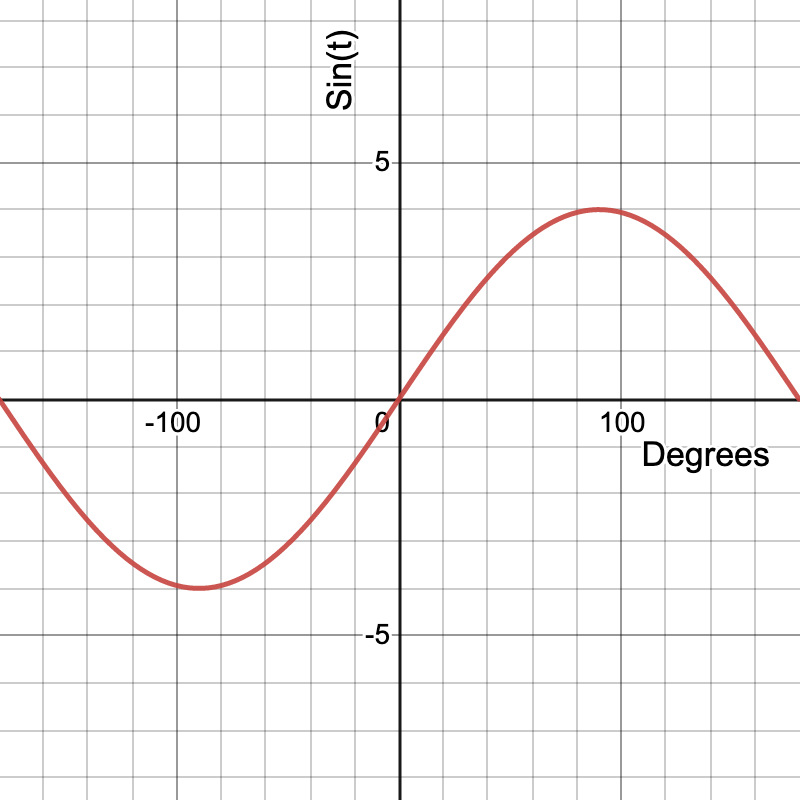
\includegraphics[width=0.40\columnwidth]{sine.png}
   \label{fig:sine}
 }
\hspace{0.2in}
\subfigure[cosine function]{
   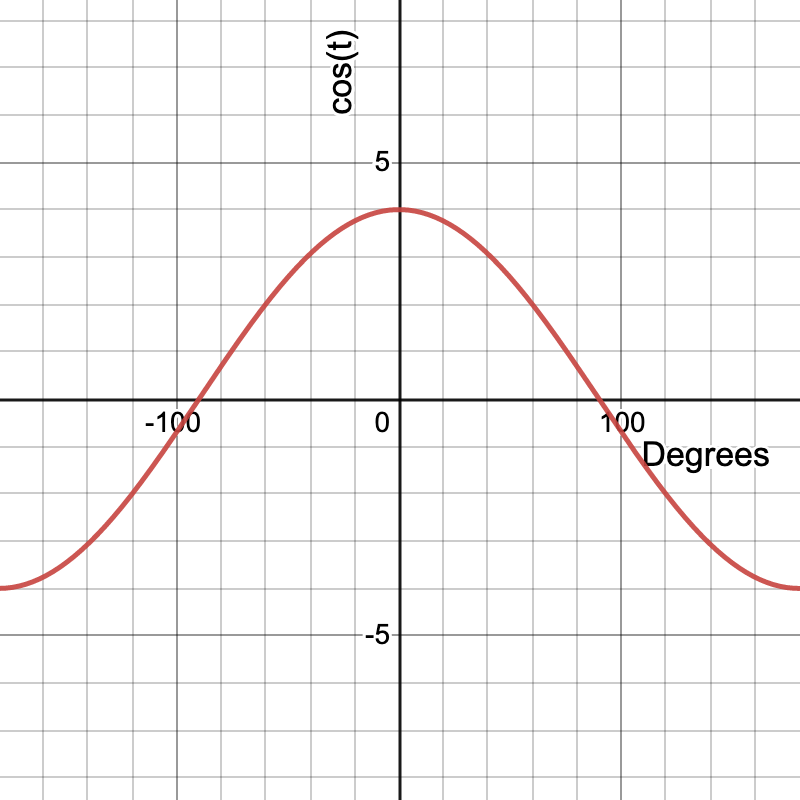
\includegraphics[width=0.40\columnwidth]{cosine.png}
   \label{fig:cosine}
 }
\end{center}
\caption{\small Examples of an odd function (left subfigure) and an even function (right subfigure).  The $\sin{(t)}$ function is odd,  with $\sin{(-t)}=-\sin{(t)}$, while the $\cos{(t)}$ function is even, with $\cos{(-t)}=\cos{(t)}$.}
\label{fig:sinusoids}
\end{figure}
\fi


\end{flushleft}
\end{document}